%% ProcessMusic.tex
%% V0.1
%% 2012/10/23
%% by Kyle Kastner
%%
%% requires IEEEtran.cls version 1.7 or later
%% This file based on content from http://www.ctan.org/tex-archive/macros/latex/contrib/IEEEtran/

\documentclass[journal]{IEEEtran}
\usepackage[labelfont=bf]{caption}
\captionsetup[figure]{labelformat=parens}
\usepackage{graphicx}
\usepackage{amsmath}
\usepackage{flushend}
\newcommand\numberthis{\addtocounter{equation}{1}\tag{\theequation}}
\begin{document}
\title{Probabilistic Matrix Factorization Methods}

\author{Kyle Kastner\\University of Texas-San Antonio}

\maketitle

\begin{abstract}
Probabilistic matrix factorization is a recent development in the field of sparse matrix factorization methods, developed partially to address issues
in modern recommender systems. Kernelized probabilistic matrix factorization offers tuneable model extensions to the probabilistic matrix
factorization framework, allowing for models which incorporate prior information about the connections between available measurements.
\end{abstract}
% IEEEtran.cls defaults to using nonbold math in the Abstract.
% This preserves the distinction between vectors and scalars. However,
% if the journal you are submitting to favors bold math in the abstract,
% then you can use LaTeX's standard command \boldmath at the very start
% of the abstract to achieve this. Many IEEE journals frown on math
% in the abstract anyway.

% Note that keywords are not normally used for peerreview papers.
\begin{IEEEkeywords}
Matrix factorization, adjacency graph, matrix kernel, recommender systems, prediction, machine learning 
\end{IEEEkeywords}

\IEEEpeerreviewmaketitle
\section{Introduction}
\IEEEPARstart{M}{atrix} factorization methods have recently gained attention in the machine learning community, due to their unique advantages sparse 
matrix recommender systems. These innovations have been fueled, at least in part, by the growing needs of social networks and online content providers to
provide customized product recommendations on a per user basis. By taking a sparse matrix \begin{math}A\end{math} as input, and attempting to 
factorize the measured values into "factors" which describe attributes of each row, \begin{math}U\end{math}, and factors of each 
column, \begin{math}V\end{math}, it is possible to estimate a value for an 
unmeasured matrix entry \begin{math}A_{i,j}\end{math} by taking the vector product of the corresponding entries \begin{math} U_i V_j^T
\end{math}. 

This paper will discuss three methods of performing this matrix decomposition: singular value decomposition (SVD), 
probabilistic matrix factorization (PMF), and kernelized probabilistic matrix factorization (KPMF). Implementation details and comparisons between
the three methods will also be discussed.

\section{Testing Data}
For evaluating the performance of each of these algorithms, the classic Lena image was used. This image was then converted into a sparse matrix via 
rejection sampling. For testing, sparseness \begin{math}s = .75\end{math} was chosen. Though these algorithms are not specifically designed to operate on 
images, this format is very convenient for qualitative inspection of algorithmic performance. Root mean square error (RMSE \cite{RMSE},
Eq. \ref{eq:RMSE}) is also used as a quantitative comparison metric.
\begin{equation}
    RMSE=\sqrt{\frac{\sum\limits^N_{n=1}(x_n-\tilde{x}_{n})^2}{N}}
\label{eq:RMSE}
\end{equation}
A visual representation of the tesing data can be seen in Fig. \ref{fig:lena} and \ref{fig:sparselena}.
\begin{figure}[h!]
\centering
    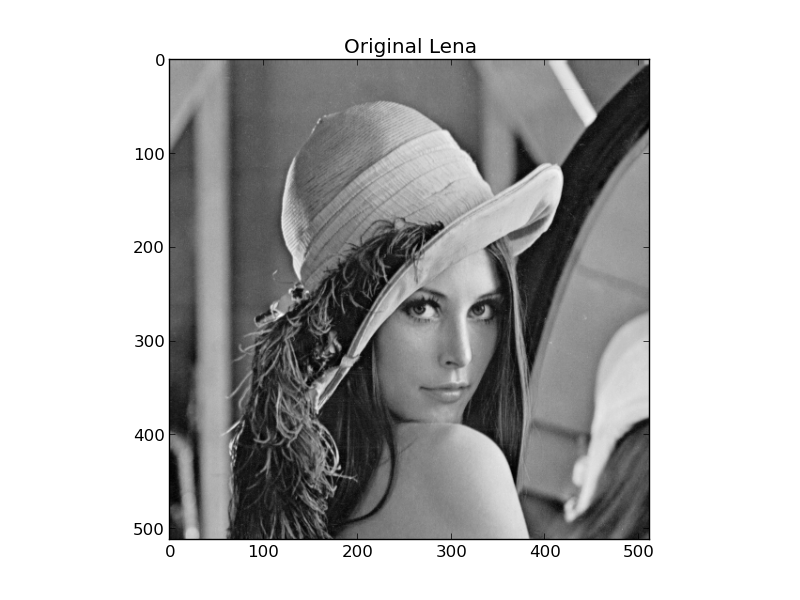
\includegraphics[width=0.45\textwidth]{lena.png}
    \caption{Full matrix Lena image data}
    \label{fig:lena}
\end{figure}
\begin{figure}[h!]
\centering
    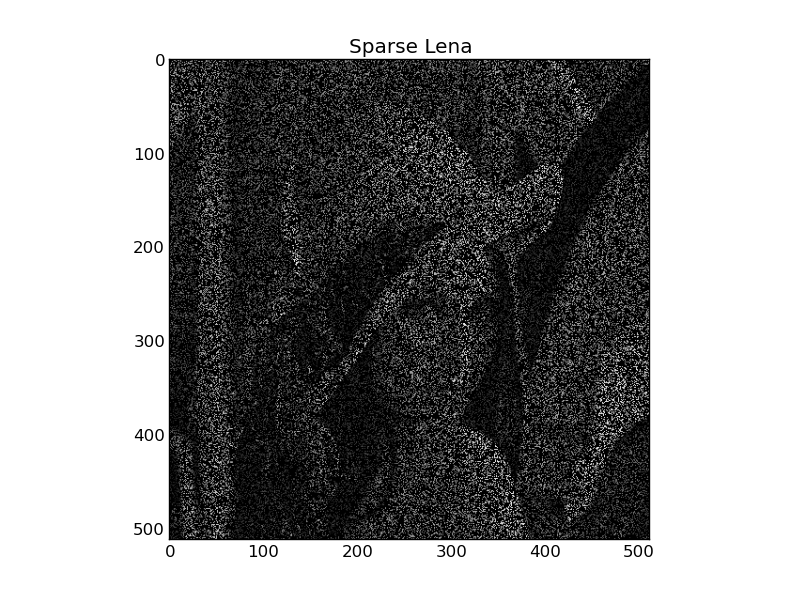
\includegraphics[width=0.45\textwidth]{sparselena.png}
    \caption{Sparse matrix Lena image data}
    \label{fig:sparselena}
\end{figure}

\section{SVD}
The SVD is a very well known technique in linear algebra, statistics, and signal processing. The SVD is based on eigendecomposition, and is often used 
in a similar manner as principal component analysis (PCA) and linear discriminant analysis (LDA), in order to decompose a matrix into 
orthogonal basis vectors that describe the row and column components. The goal of SVD is to find a solution to Eq. \ref{eq:SVD} \cite{SVDIntuition}.
\begin{equation}
    A=U \Sigma V^T
\label{eq:SVD}
\end{equation}
There are many formulas for the numerical calculation of the SVD, though one of the most common methods used is the Lanczos
algorithm. The reference implementation for this paper used Python, with the scipy and numpy libraries. These Python libraries in turn used 
the ARPACK FORTRAN library, which implements the Lanczos algorithm in order to perform the SVD computation \cite{SCIPYsource} \cite{ARPACKsource}. 
The SVD was originally developed for full-matrix decomposition, but it also functions for sparse matrices. 
The resultant matrices \begin{math}U,V\end{math} are of dimension \begin{math}N \times K\end{math} and \begin{math}K \times N\end{math} respectively, where the number of support parameters
\begin{math}K\end{math} allows for a tradeoff between computational complexity and reconstruction quality. All computations in this experiment used
\begin{math}K=10\end{math} for the number of factors per row and column element. Evaluating the SVD on the full and sparse matrix Lena datasets led to 
Fig. \ref{fig:fullSVD} and \ref{fig:sparseSVD} All algorithms were also evaluated with the number of repetitions \begin{math}R = 7\end{math}.
\begin{figure}[h!]
\centering
    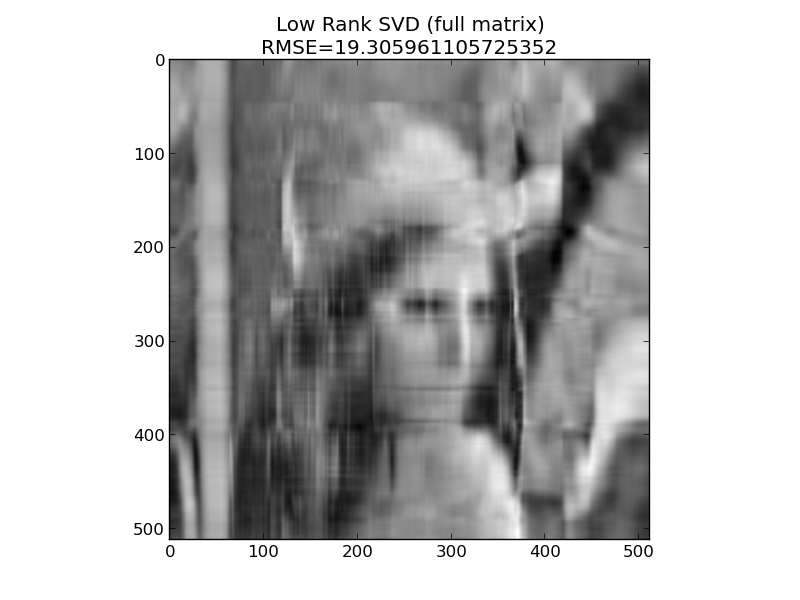
\includegraphics[width=0.45\textwidth]{fullsvd.png}
    \caption{Full matrix SVD}
    \label{fig:fullSVD}
\end{figure}
\begin{figure}[h!]
\centering
    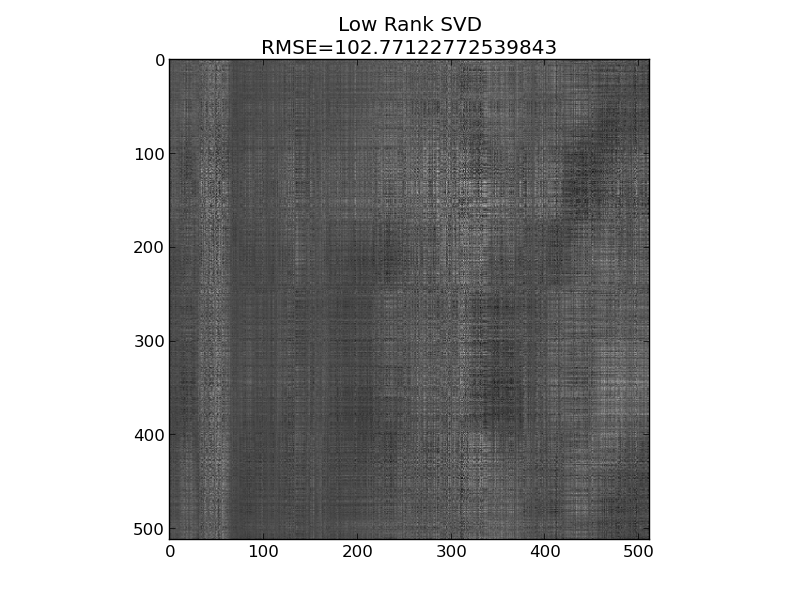
\includegraphics[width=0.45\textwidth]{sparsesvd.png}
    \caption{Sparse matrix SVD}
    \label{fig:sparseSVD}
\end{figure}

\section{PMF}
Next, the sparse Lena dataset was evaluated using probabilistic matrix factorization, or PMF. PMF was developed in response to the Netflix
recommendation algorithm competition. This compeition was initiated to find the best recommendation algorithm for Netflix users, 
given an existing sparse matrix of user, movie recommendations \begin{math}A_{i,j}\end{math}, rows \begin{math}i \in N\end{math} representing movies, 
and columns \begin{math}j \in M\end{math}
representing users. The subsequent decomposition of \begin{math}A\end{math} results in a matrix of user factors \begin{math}U\end{math}, and a matrix of
movie factors \begin{math}V\end{math}. These matrices have \begin{math}dim(U) = N \times K \end{math}, and \begin{math}dim(V) = K \times M\end{math},
with original matrix \begin{math}dim(A) = N \times M\end{math}. From the log posterior probability given in \cite{PMFpaper}, the decomposition of
\begin{math}A\end{math} into \begin{math}U\end{math} and \begin{math}V\end{math} is achieved by minimizing the error function shown in Eq. \ref{eq:PMFerr}.
\begin{align}
    E=\frac{1}{2}\sum\limits_{i=1}^N\sum\limits_{j=1}^MI_{i,j}(A_{i,j}-U_iV_j^T)^2 \nonumber \\
    +\frac{\lambda_U}{2}\sum\limits_{i=1}^N||U_i||_{Fro}^2 \nonumber \\
    + \frac{\lambda_V}{2}\sum\limits_{j=1}^M||V_j||_{Fro}^2
\label{eq:PMFerr}
\end{align}
In these functions, \begin{math}I_{i,j}\end{math} is an indicator value to represent the presence of a measurement in the sparse matrix, with 
\begin{math}I_{i,j} \in \left\{0,1\right\} \end{math}.
To minimize this error function, the general gradient descent algorithm is applied iteratively, using the set of equations in Eq. \ref{eq:PMFgrad},
choosing learning rate \begin{math}\alpha = .001\end{math}, and iterating through values 
\begin{math}\lambda_U = \lambda_V \in \left\{0,.25,.5,.75,1\right\}
\end{math}.
\begin{equation}
    V_{i,j} = V_{i,j} - \alpha\frac{\partial E}{\partial V} \nonumber
\end{equation}
\begin{equation}
    U_{i,j} = U_{i,j} - \alpha\frac{\partial E}{\partial U} \nonumber
\end{equation}
\begin{equation}
    \frac{\partial E}{\partial V} = -\sum\limits_{i=1}^N\sum\limits_{j=1}^MI_{i,j}(A_{i,j}-U_i^TV_j)U_i^T + \lambda_V\sum\limits_{j=1}^MV_j \nonumber \\
\end{equation}
\begin{equation}
    \frac{\partial E}{\partial U} = -\sum\limits_{i=1}^N\sum\limits_{j=1}^MI_{i,j}(R_{i,j}-U_i^TV_j)V_j + \lambda_U\sum\limits_{i=1}^NU_i
    \label{eq:PMFgrad}
\end{equation}
The results applying PMF to the sparse Lena dataset are shown in Fig. \ref{fig:sparsepmf}.
\begin{figure}[h!]
\centering
    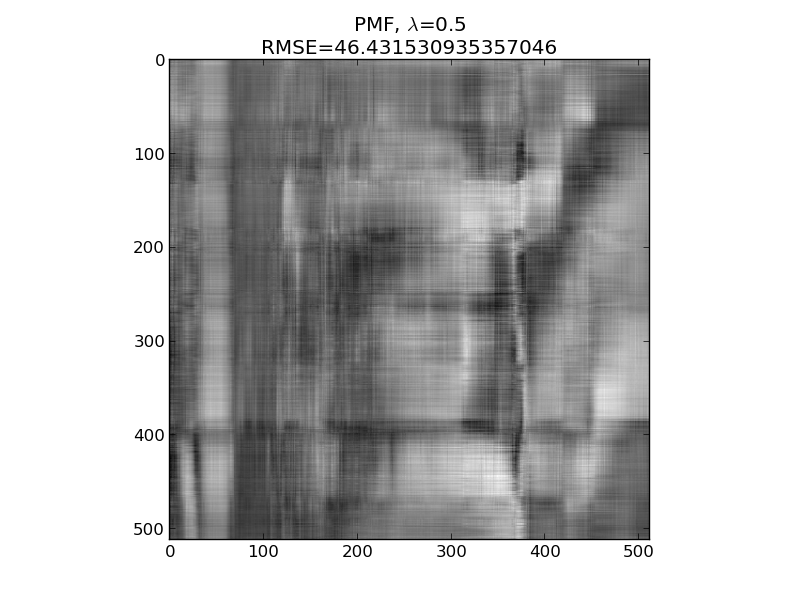
\includegraphics[width=0.45\textwidth]{sparsepmf.png}
    \caption{Sparse matrix PMF}
    \label{fig:sparsepmf}
\end{figure}

\section{KPMF}
KPMF, or kernelized probabilistic matrix factorization, is an extension of the PMF algorithm described above. A full derivation can be seen in 
\cite{KPMFpaper}, but key additions of the KPMF algorithm over PMF are: minimizing a different error function, adding an additional adjacency 
matrix term to describe the connections between matrix entries, and adding a customizable kernel to describe the strength of these connections. The last
two modifications allow the incorporation of side information such as social models, spatial models, or custom models for domain specific
problems. This increases the number of free parameters in a problem, but can allow for stronger estimates when measurements are 
extremely sparse. KPMF is accomplished by minimizing Eq. \ref{eq:KPMFerr}.
\begin{align}
    E=\frac{1}{2}\sum\limits_{i=1}^N\sum\limits_{j=1}^MI_{i,j}(A_{i,j}-U_iV_j^T)^2 \nonumber \\
    +\frac{\lambda_U}{2}\sum\limits_{i=1}^NU^T_iS_UU_i \nonumber \\
    + \frac{\lambda_V}{2}\sum\limits_{j=1}^MV^T_jS_VV_j
\label{eq:KPMFerr}
\end{align}
This error function is again minimized using gradient descent, resulting in Eq. \ref{eq:KPMFgrad}. Results were generated by choosing learning rate 
\begin{math}\alpha = .001\end{math}.
\begin{equation}
    V_{i,j} = V_{i,j} - \alpha\frac{\partial E}{\partial V} \nonumber
\end{equation}
\begin{equation}
    U_{i,j} = U_{i,j} - \alpha\frac{\partial E}{\partial U} \nonumber
\end{equation}
\begin{equation}
    \frac{\partial E}{\partial V} = -\sum\limits_{i=1}^N\sum\limits_{j=1}^MI_{i,j}(A_{i,j}-U_i^TV_j)U_i^T + \lambda_V\sum\limits_{j=1}^MS_VV_j \nonumber \\
\end{equation}
\begin{equation}
    \frac{\partial E}{\partial U} = -\sum\limits_{i=1}^N\sum\limits_{j=1}^MI_{i,j}(R_{i,j}-U_i^TV_j)V_j + \lambda_U\sum\limits_{i=1}^NS_UU_i
    \label{eq:KPMFgrad}
\end{equation}
Most of the terms in Eq. \ref{eq:KPMFgrad} are shared with the derivation of the PMF in Eq. \ref{PMFgrad}, however new terms have emerged: 
\begin{math}S_U, S_V\end{math}. These terms represent precision matrices associated with a generated kernel. There are many different methods for
generating the kernel matrix, as seen in \cite{KPMFpaper}, but for image applications, the authors indicate a preference for the diffusion
kernel. To generate a diffusion kernel (and its precision \begin{math}S)\end{math}, begin by creating a band matrix of bandwidth \begin{math}W\end{math},
which describes how many rows and columns can be considered connected. Various bandwidths were tested during this research, but bandwidth 
\begin{math}2\Delta = W = 10\end{math} is listed in \cite{KPMFpaper}. Generating matrix \begin{math}C\end{math}, it is next necessary to calculate
the degree matrix \begin{math}D\end{math} of \begin{math}C\end{math}, by summing the columns of \begin{math}C\end{math} and placing the sum on the 
diagonal, in order to calculate the graph laplacian \cite{Laplacian}.
\begin{equation}
    L = D - C
\end{equation}
With the Laplacian calculated, the next step is to apply the diffusion equation 
\begin{equation}
K = e^{-\beta L}
\label{eq:diffusion}
\end{equation}
\begin{math}\beta\end{math} is a chosen contant for the strength of connection between adjacent rows and columns. 
\begin{math}\beta = .5\end{math} was used for this reseach.
It is important to note that Eq. \ref{eq:diffusion} uses the matrix exponential, not element by element exponentiation. 
These operations result in a final matrix 
\begin{equation}
K = K_U = K_V
\end{equation}
\begin{equation}
S = S_U = S_V = K^{-1}
\end{equation}
\begin{figure}[h!]
\centering
    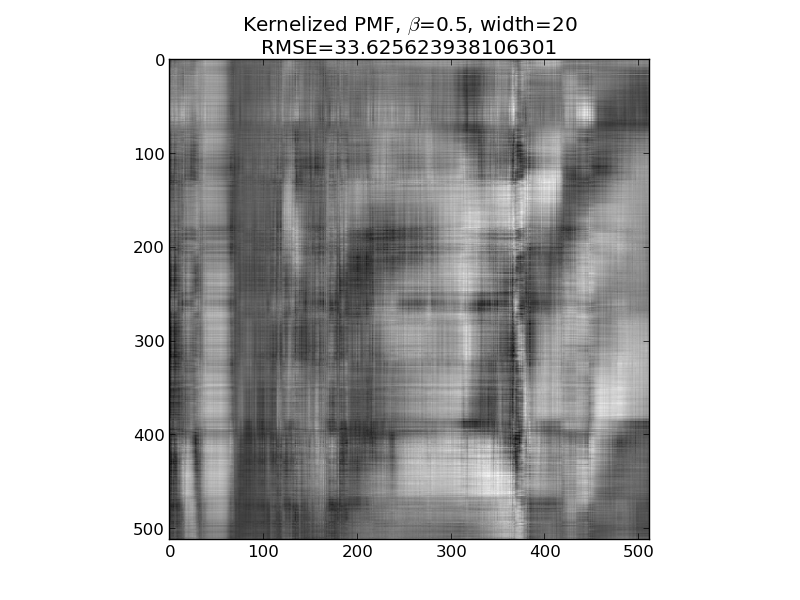
\includegraphics[width=0.45\textwidth]{sparsekpmf.png}
    \caption{Sparse matrix KPMF}
    \label{fig:sparsekpmf}
\end{figure}

\section{Results}
The resulting RMSE values for PMF and KPMF calculations are shown in Figs. \ref{fig:kernelrmse} and \ref{fig:regdiffrmse}. KPMF shows notable improvement over
PMF, but a thorough search for optimized paramaters would likely yield better results for both algorithms.
\begin{figure}[h!]
\centering
    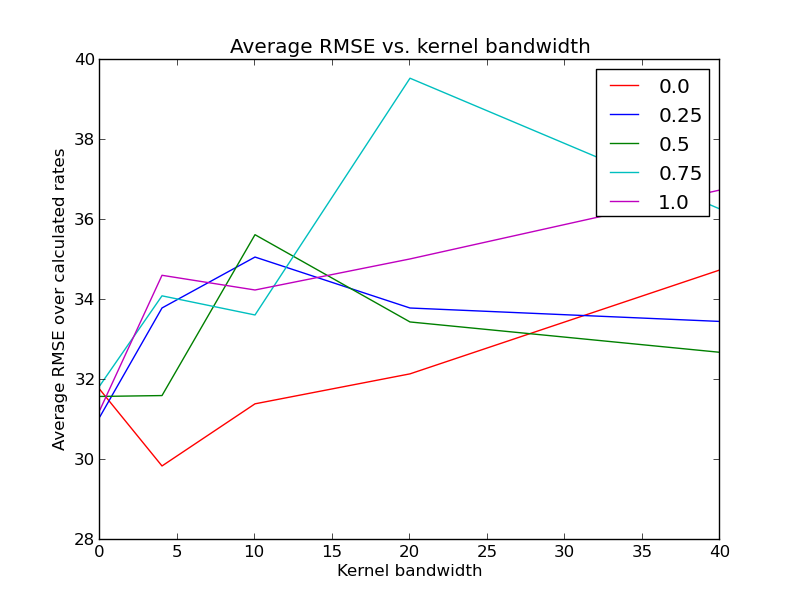
\includegraphics[width=0.45\textwidth]{kernelrmse.png}
    \caption{Kernel bandwidth RMSE}
    \label{fig:kernelrmse}
\end{figure}
\begin{figure}[h!]
\centering
    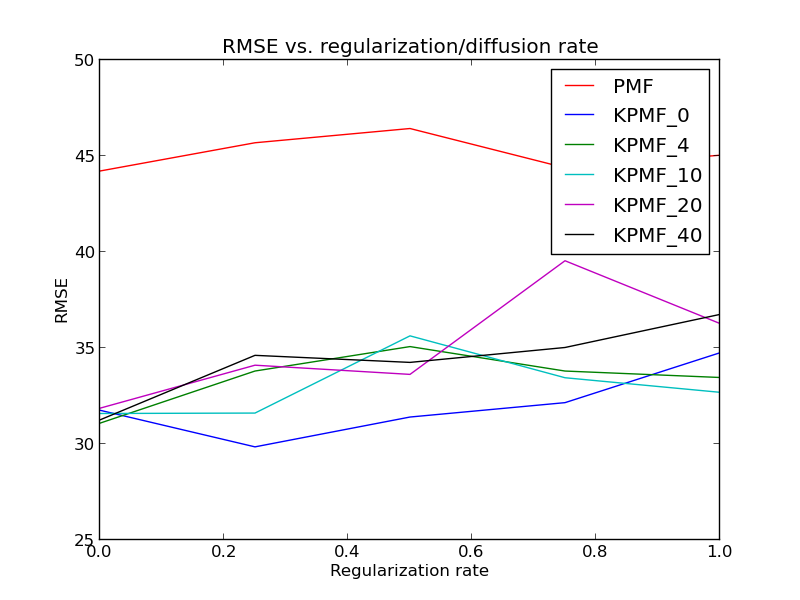
\includegraphics[width=0.45\textwidth]{regdiffrmse.png}
    \caption{KPMF and PMF RMSE Comparison}
    \label{fig:regdiffrmse}
\end{figure}

\section{Comparison}
In earlier sections, only the prediction output of each algorithm is shown. For images, an extra step can be taken by combining the sparse input and 
prediction output. If there exists a measured value, it is preferred over the estimation of the algorithm. Everywhere else, the algorithmic prediction
results are preferred. Combining in this way, Figs. \ref{fig:combinedsparsesvd}, \ref{fig:combinedpmf}, and \ref{fig:combinedkpmf} show
visual improvement.
\begin{figure}[h!]
\centering
    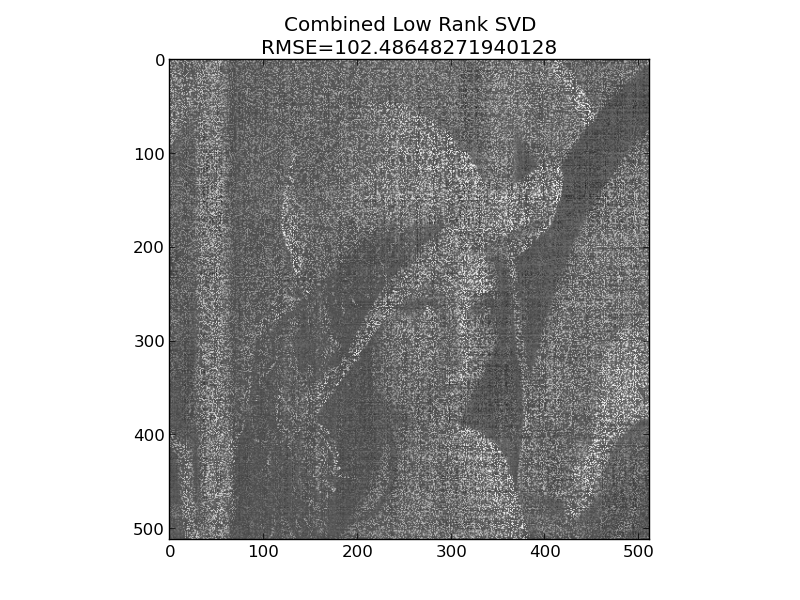
\includegraphics[width=0.45\textwidth]{combinedsparsesvd.png}
    \caption{Combined sparse matrix SVD}
    \label{fig:combinedsparsesvd}
\end{figure}
\begin{figure}[h!]
\centering
    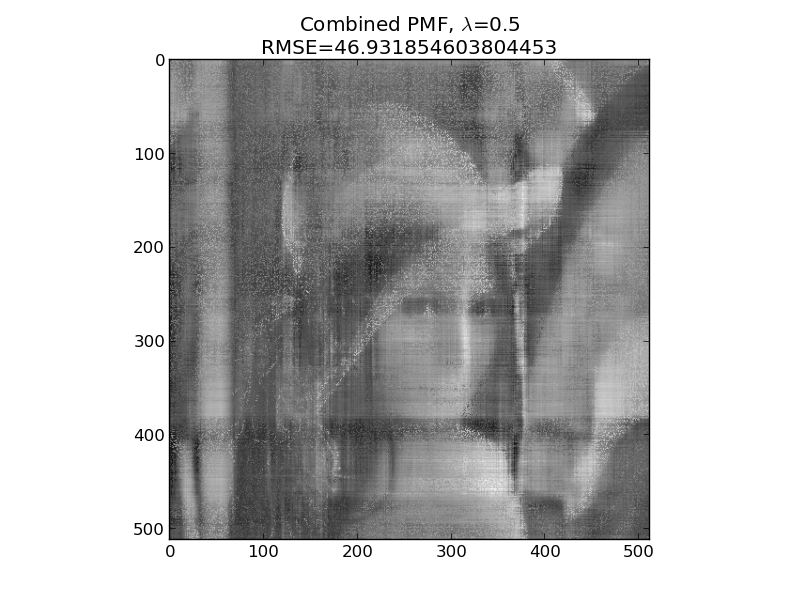
\includegraphics[width=0.45\textwidth]{combinedpmf.png}
    \caption{Combined sparse matrix PMF}
    \label{fig:combinedpmf}
\end{figure}
\begin{figure}[h!]
\centering
    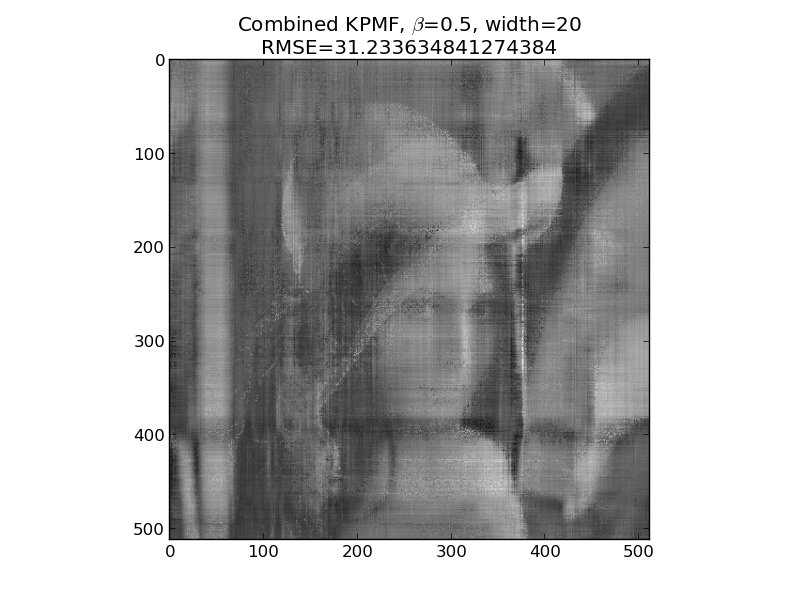
\includegraphics[width=0.45\textwidth]{combinedkpmf.png}
    \caption{Combined sparse matrix KPMF}
    \label{fig:combinedkpmf}
\end{figure}
%\subsection{Notes}
%\begin{equation}
%    x_q = x_n + e_n
%\end{equation}
%\begin{thebibliography}{1}
%
%\begin{figure}[h!]
%\centering
%  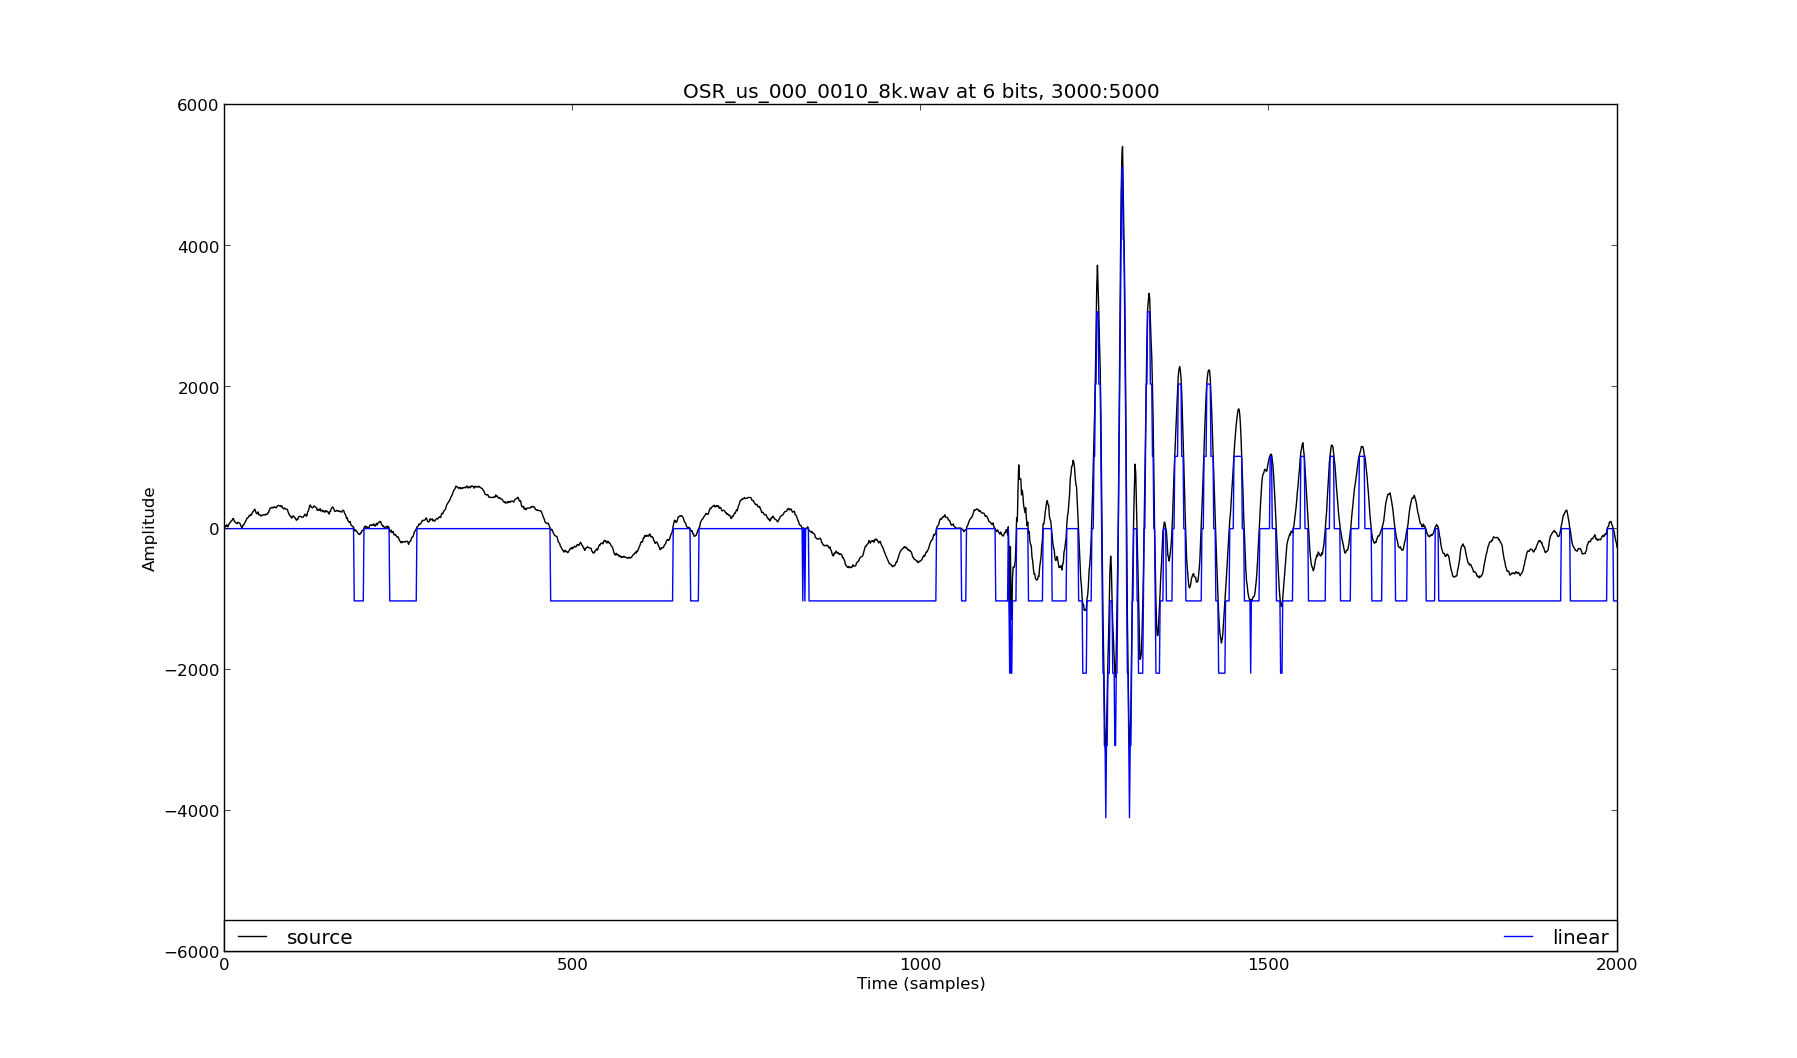
\includegraphics[width=0.45\textwidth]{linear_6bit.png}
%\caption{Linear quantization, $B = 6$}
%\label{fig:linear}
%\end{figure}
%\ref{fig:linear}

\vfill
\vfill
\vfill
\begin{thebibliography}{1}
\bibitem{RMSE}
Unknown Author, \emph{Root Mean Square Error}. Taken from http://www.ctec.ufal.br/professor/crfj/\\
Graduacao/MSH/Model\%20evaluation\%20methods.doc, on May 10, 2013.
\bibitem{SVDIntuition}
Unknown Author, \emph{The Singular Value Decomposition in Symmetric Orthogonalization and Data Compression}.
Taken from http://www.wou.edu/~beavers/Talks/Willamette1106.pdf, on May 10, 2013.
\bibitem{SCIPYsource}
SciPy community, \emph{Sparse Eigenvalue Problems with ARPACK}. 
Taken from http://docs.scipy.org/doc/scipy/reference/tutorial/arpack.html, on May 10, 2013.
\bibitem{ARPACKsource}
R. Lehoucq, K. Maschhoff, D. Sorensen, C. Yang, \emph{ARPACK Documentation}. Taken from http://www.caam.rice.edu/software/ARPACK/, on May 10, 2013.
\bibitem{PMFpaper} 
R. Salakhutdinov, A. Mnih, \emph{Probabilistic Matrix Factorization}. Taken from http://www.cs.utoronto.ca/~amnih/papers/pmf.pdf, on May 10, 2013.
\bibitem{KPMFpaper}
T. Zhou, H. Shan, A. Banerjee, G. Sapiro, \emph{Kernelized Probabilistic Matrix Factorization: Exploiting Graphs and Side Information}. 
Taken from http://www.ece.duke.edu/~lcarin/kpmf\_sdm\_final.pdf, on May 10, 2013.
\bibitem{Laplacian}
R. Horaud, \emph{A Short Tutorial on Graph Laplacians, Laplacian Embedding, and Spectral Clustering}. Taken from 
http://csustan.csustan.edu/~tom/Clustering/GraphLaplacian-tutorial.pdf, on May 10, 2013.
\end{thebibliography}

% You can push biographies down or up by placing
% a \vfill before or after them. The appropriate
% use of \vfill depends on what kind of text is
% on the last page and whether or not the columns
% are being equalized.

%\vfill

% Can be used to pull up biographies so that the bottom of the last one
% is flush with the other column.

\enlargethispage{-5in}
% that's all folks
\end{document}


